%Contribution Section
\section{Velocity of money in effective circulation}
\label{sec:newmeas}%
%
While these measures advanced quantifying the velocity of cryptocurrencies,
they suffer from inaccuracy as money supply is defined as ``the aggregate of
all monetary units ever issued'' ($\MTotalP$).  We therefore propose a
measure based on the component of money that circulates effectively. %
Denoting this circulating amount $\MCircP$, our measure yields
\begin{align}%
  \label{eq:vcirc_concept}
  \VCircEstP = \frac{\langle\Pp,\Tp\rangle}{\MCircP}.%
\end{align}%
%
% $\VCircP$ handles re-activated money gracefully, allowing %
% for a deeper glance into the economics of the cryptocurrency markets. %
% If money supply responds to price trends, not only numerator but also %
% denominator change. %
% For more or less money in potentially being available for transactions, %
% $\VCircP$ reflects, whether this money indeed has been %
% used for processing transactions and to which degree. %

\subsection{Formal derivation}
\label{sec:formal-derivation}

To see how excluding hoarded money relates to the quantity theory, expand the
sum in \refequ{velo_concept} and differentiate the set of all monetary units
treated as investment, $h$, from its complement
$\GStrokeP\coloneqq\Gp\setminus\{h\}$:
\begin{alignat}{4}%
  \VTotalP%
  \ & = &\ & \vp_h \frac{%
    \Np_h%
  }{%
    \bigl( \Np_h+\sum_{g\in\GStrokeP} \Np_g \bigr)%
  }\\%
  \ & \ + &\ & \sum_{g\in\GStrokeP} \vp_g \frac{%
    \Np_g%
  }{%
    \bigl( \Np_h+\sum_{g\in\GStrokeP} \Np_g \bigr)%
  }.\nonumber%
\end{alignat}%
%
By definition, $h$ encompasses only non-transferred units, and thus $\vp_h=0$
in period $\perd$. Consequently %
% For a large fraction of money supply $\Np_z=0$ held %
% as investment, the respective turnover rate $\vp_z$ receives a %
% large weight %
% \begin{align}
% \frac{\Np_z}{\bigl( \Np_z+\sum_{g\in\GStrokeP} \Np_g \bigr)},
% \end{align} %
% while the components of actively used money supply receive a %
% small weight. %
% Velocity measured in the above way %
% thus yields values close to zero, making the variable slightly abstract in its %
% interpretation. %

% Money switching from \textit{hoarded} to \textit{in circulation} %
% increases or decreases the measure. %
% Thus, a change in the measure $\VTotalEstP$ could either mean that "effectively %
% circulating monetary units on average being turned over more times" or %
% "formerly illiquid monetary units are being now used for transactions". %
% %
% Measure $\VCircP$ reduces the equation to% 
\begin{align}%
  \label{eq:disentangle_vcirc}
  \VCircP %
  =  \sum_{g\in\GStrokeP} \vp_g
  \frac{\Np_g}{\sum_{g\in\GStrokeP} \Np_g },%
\end{align}%
% where group $h$, hoarded money, is not considered.
% , an interpretation of a change in $\VCircP$ can here clearly %
% be attributed to a higher intensity of turnover for the circulating money stock. %
% Assuming that self-churn transactions in the calculation of %
% the transaction volumes have been filtered out effectively, the measure %
% might be interpreted as a proxy for the %
% \textbf{average number of peer-to-peer hops that effectively circulating %
% 	money units where able to achieve} in period $\perd$. 
Hence, the measure can be interpreted as the average number of turnovers of
units effectively circulating in period $\perd$. %
Dropping non-circulating money in \refequ{disentangle_vcirc} amounts to an
adjustment of the money supply $\Mp$ in the quantity equation
\eqref{eq:fisher}.  %

\subsection{Theoretical basis and practical considerations}
An advantage of basing velocity on money in effective circulation is higher
information content. %
To begin with, it is questionable whether $\VNaiveEst$ and $\VTotalEst$
capture more information than transaction volumes $\langle\Pp,\Tp\rangle$,
respectively $\langle\Pp',\Tp'\rangle$. %
After all, for most UTXO-based cryptocurrencies money supply is just a simple
function of block height.%
\footnote{Difficulty adjustments for mining lead to close-to-constant spans
  between block creation times \citep{tschorsch2016bitcoin}.} %
% So far, there are only few cryptocurrencies that implement a responsive %
% money supply.%
% \footnote{%
%   Some so called ``stablecoins'' developed with the goal of a more stable %
%   purchasing power are trying to implement a coin supply matching the %
%   demand (compare \cite{klages2019stability}, \cite{routledge2018currency}, %
%   \cite{sidorenko2019stablecoin} \cite{pernice2019monetary} or \cite{bullmann2019search}).%
% } %
Thus, the two former measures appear very close to merely scaled versions of
their price-sums. %

Moreover, the total coin supply used in $\VNaiveEst$ and $\VTotalEst$
includes money that is technical dysfunctional (burnt coins). %
Yet also coins held unused as storage of wealth\footnote{Compare
  \cite{sawyer2003money} for a detailed discussion of the discrepancy arising
  from money as storage of wealth.} %
or speculation\footnote{Most studies conclude cryptocurrencies are currently used more for
  long-term speculation rather than as media of exchange %
  (see \eg \cite{%
    bouri2019herding,%
    anderson2019bitcoin,%
    yang2018behavioral,%
    yermack2015bitcoin%
  }).
  % The degree to which monetary units are hold unused can be %
  % seen e.g. in \cite{kalodner2017blocksci}, who find that over the last 10 years only roughly %
  % \SI{20}{\percent} of Bitcoins were %
  % spent again within a month. %
} %
do not fulfill one of the key functions of money, use as medium of exchange.%
\begin{figure*}[ht!]%
	\centering
	\ifdefined\varInputFigs%
%	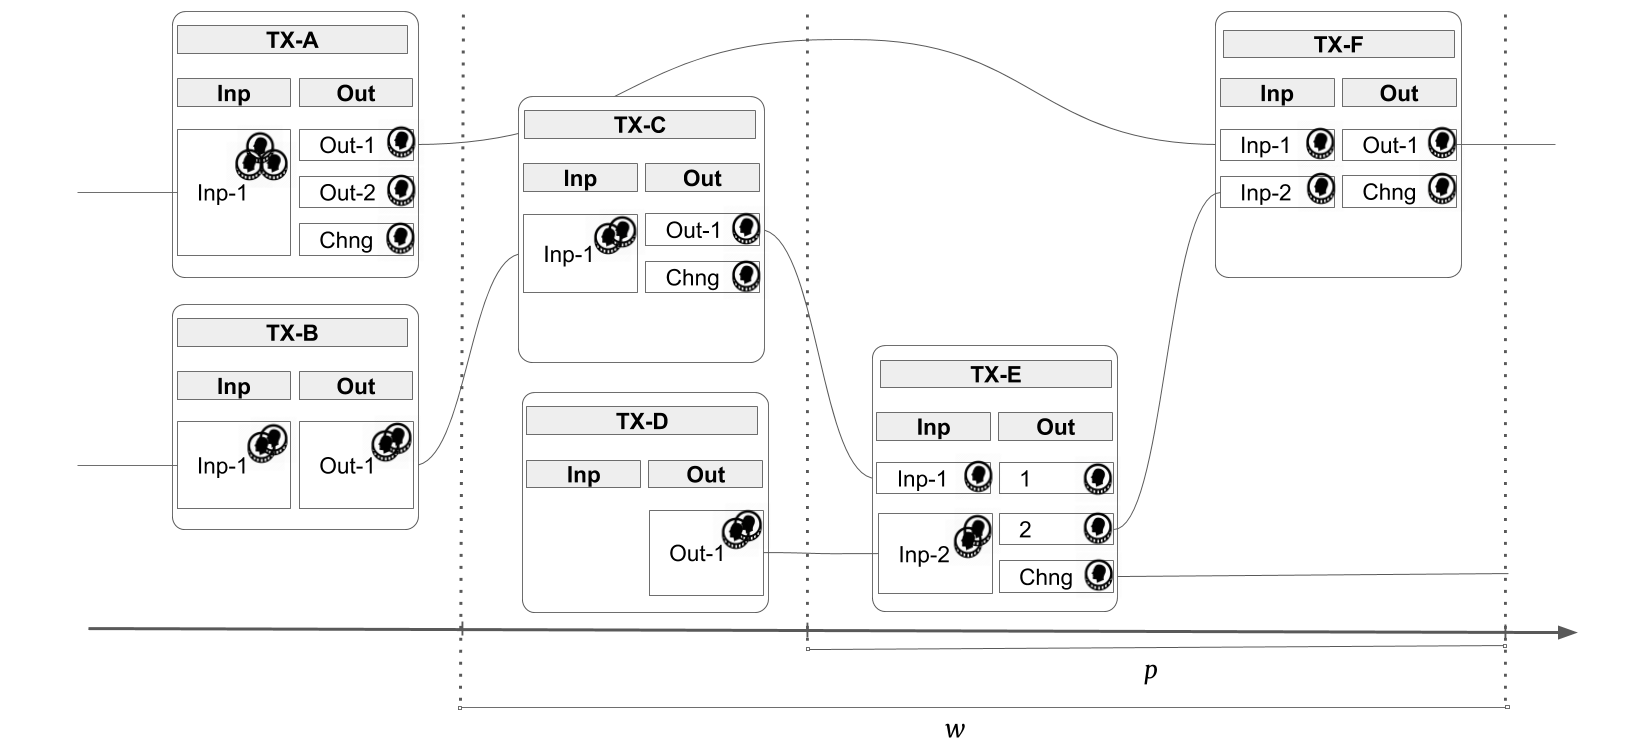
\includegraphics[width=0.8\linewidth]{fig/mcirc_concept_window_uneqal_period_HR}%
	%-------------------------------------------------------------------------------
\usetikzlibrary{calc}
%coordinate test point. Use as follows: 	\coordinate (cen) 	 	 at (0,0) (cen) [point];
\tikzset{
	every point/.style = {radius={\pgflinewidth}, opacity=1, draw, solid, fill=white},
	pt/.pic = {
		\begin{pgfonlayer}{foreground}
			\path[every point, #1] circle;
		\end{pgfonlayer}
	},
	point/.style={insert path={pic{pt={#1}}}}, point/.default={},
	point name/.style = {insert path={coordinate (#1)}}
}
%-------------------------------------------------------------------------------

% basic delacations
\pgfdeclarelayer{background}%
\pgfdeclarelayer{foreground}%
\pgfsetlayers{background,main,foreground}%

%Coin Symbol--------------------------------------------------------------------
\tikzset{%
	pics/coin/.style n args={3}{%
		code ={
			\def \coinLineWidth {#1}%
			\def \coinCenDist   {#2}%
			\def \circRad       {#3}%
			\def \signRad       {\circRad*0.20}%
			\def \signRadProp   {0.45}
			\def \signRadExt    {\signRad*\signRadProp}
			\def \signRadOut    {\signRad+\signRadExt}
			\def \signAngle     {30}
			\def \sinSignAngle  {sin(\signAngle)}
			\def \cosSignAngle  {cos(\signAngle)}
			\def \signWidth     {{pow((pow(\signRadOut,2)-pow(\sinSignAngle*\signRad,2)),0.5)-(\cosSignAngle)*\signRad)}}
			
			\def \startIX       {{cos(\signAngle)*\signRad}}
			\def \startIY       {{\sinSignAngle*\signRad}}
			
			\def \startOY       {\startIY}
			\def \signAngleOutS {{atan((\sinSignAngle*\signRad)/pow((pow(\signRadOut,2)-pow(\sinSignAngle*\signRad,2)),0.5))}}
			\def \signAngleOutE {{360-atan((\sinSignAngle*\signRad)/pow((pow(\signRadOut,2)-pow(\sinSignAngle*\signRad,2)),0.5))}}
	%
			\coordinate ()          at ( 0.0     , 0.0);%
			\coordinate (cen)       at ( 0.0     , 0.0);%
			\coordinate (cenB)      at ($(cen)    + ( 0.00,-\coinCenDist)$);%
						
			\node[
				circle,
				draw = black,
				fill = white,
				line width = \coinLineWidth,
				minimum size = \circRad,
				inner sep = 0pt,
				outer sep = 0pt,
			](NCD) at (cenB) {};
			
			\node[
				circle,
				draw = black,
				fill = white,
				line width = \coinLineWidth,
				minimum size = \circRad,
				inner sep = 0pt,
				outer sep = 0pt,
			](NCU) at (cen) {};
			
%			\draw[ - , line width = \coinLineWidth, black] (NCU.195) -- (NCD.195);
			\draw[-, line width = \coinLineWidth, black] (NCU.210) -- (NCD.210);
			\draw[-, line width = \coinLineWidth, black] (NCU.225) -- (NCD.225);
			\draw[-, line width = \coinLineWidth, black] (NCU.240) -- (NCD.240);
			\draw[-, line width = \coinLineWidth, black] (NCU.255) -- (NCD.255);
			\draw[-, line width = \coinLineWidth, black] (NCU.270) -- (NCD.270);
			\draw[-, line width = \coinLineWidth, black] (NCU.285) -- (NCD.285);
			\draw[-, line width = \coinLineWidth, black] (NCU.300) -- (NCD.300);
			\draw[-, line width = \coinLineWidth, black] (NCU.315) -- (NCD.315);
			\draw[-, line width = \coinLineWidth, black] (NCU.330) -- (NCD.330);
%			\draw[ - , line width = \coinLineWidth, black] (NCU.345) -- (NCD.345);
			
			\draw[
				 - ,
				 line width = \coinLineWidth,
				 black!80!white,
				 fill = black!80!white
			]
				(\startIX,-\startIY) arc (360-\signAngle:\signAngle:\signRad)
				-- +(\signWidth, 0.0)
				arc (\signAngleOutS:\signAngleOutE:\signRadOut)
				-- (\startIX,-\startIY)
				-- cycle
				;
		}%
		
	} ,%
	pics/coin/.default={1.0pt}{0.1}{1cm}%
}%
%
\begin{tikzpicture}
	\def \debugPoint   {}%
%b	\def \debugPoint   {point}%
	% font settings ############################################################
	\def \fontset      {\scriptsize\sffamily}
	% color definition #########################################################
	\def \colorOut     {black!100!white}
	\def \colorIn      {black!10!white}
	% arrow and line definitions ###############################################
	\def \lineW        {1.3pt}
	% width/height definition ##################################################
	\def \picW         {\linewidth*25.5/31}%
	\def \picH         {\paperheight*7.75/31}%
	\def \TH           {\picH*0.4}%picH*0.5*0.8
	
	\def \WBA          {\picW*11.50/31}
	\def \WLA          {\picW* 7.75/31}
	\def \WBB          {\picW* 4.00/31}
	\def \WLB          {\picW* 0.25/31}
	\def \WBC          {\picW* 3.50/31}
	\def \WBD          {\picW*10.50/31}
	\def \WLD          {\picW*14.25/31}
	% width/height nodes/boxes###################################################
	\def \BOH          {\picH* 0.35  }
	\def \BOW          {\picW* 6.0/31}
	
	% node positioning
	\def \BIPX         {\BOW*0.2375}
	
	% tikz styles################################################################
	\tikzstyle{lineIO} = [
		- ,
		line width = \lineW*0.8,
	]
	\tikzstyle{nodeOuter}   = [
		draw,
		rectangle,
		rounded corners=5pt,
		solid,
		line width = \lineW,
		black,
		inner sep = 0pt,
		outer sep = 0pt,
		text width = \BOW,
		minimum width = \BOW,
		minimum height = \BOH*1.075,
	]
	\tikzstyle{nodeInner}   = [
		draw,
		rectangle,
		rounded corners=3pt,
		solid,
		line width = \lineW*0.9,
		black,
		fill = \colorIn,
		inner sep = 0pt,
		outer sep = 0pt,
	]
	\tikzstyle{nodeInnerA}  = [
		nodeInner,
		align = center,
		text width = \BOW*0.9-3pt,
		minimum width = \BOW*0.9,
		minimum height = \BOH*0.15,
	]
	\tikzstyle{nodeInnerB}  = [
		nodeInner,
		align = left,
		text width = \BOW*0.425-5pt,
		minimum width = \BOW*0.425,
	]
	\tikzstyle{nodeInnerBA} = [
		nodeInnerB,
		minimum height = \BOH*0.15,
	]	
	\tikzstyle{nodeInnerBAC}b= [
		nodeInnerB,
		minimum height = \BOH*0.15,
		align = center,
	]
	\tikzstyle{nodeInnerBB} = [
		nodeInnerB,
		minimum height = \BOH*0.25,
	]
	\tikzstyle{nodeInnerBC} = [
		nodeInnerB,
		minimum height = \BOH*0.35,
	]
	\tikzstyle{nodeInnerBD} = [
		nodeInnerB,
		minimum height = \BOH*0.55,
	]
	% coordinates ###############################################################
	% 1 | 2 | 3 | 4 | 5 | 6 | 7 | 8 | 9 | 10 | 11 | 12 | 13 | 14 |
	% A | B | C | D | E | F | G | H | I |  J |  K |  L |  M |  N |
	
	\coordinate (cen)       at ($(0.0,0.0)   + ( 0.0       , 0.0         )$) (cen)   [\debugPoint];%
	
	\coordinate (PLU)       at ($(cen)       + (-\picW*0.5 , \picH*0.5   )$) (PLU)   [\debugPoint];%
	\coordinate (PLD)       at ($(cen)       + (-\picW*0.5 ,-\picH*0.5   )$) (PLD)   [\debugPoint];%
	\coordinate (PRU)       at ($(cen)       + ( \picW*0.5 , \picH*0.5   )$) (PRU)   [\debugPoint];%
	\coordinate (PRD)       at ($(cen)       + ( \picW*0.5 ,-\picH*0.5   )$) (PRD)   [\debugPoint];%
	
	
	\coordinate (TC)        at ($(cen)       + ( 0.0       ,-\TH         )$) (TC)    [\debugPoint];%
	\coordinate (TL)        at ($(TC)        + (-\picW*0.5 , 0.0         )$) (TL)    [\debugPoint];%
	\coordinate (TR)        at ($(TC)        + ( \picW*0.5 , 0.0         )$) (TR)    [\debugPoint];%
	
	\coordinate (BAC)       at ($(cen)       + (-\WBA      , 0.0         )$) (BAC)   [\debugPoint];%
	\coordinate (LAC)       at ($(cen)       + (-\WLA      , 0.0         )$) (LAC)   [\debugPoint];%
	\coordinate (BBC)       at ($(cen)       + (-\WBB      , 0.0         )$) (BBC)   [\debugPoint];%
	\coordinate (LBC)       at ($(cen)       + (-\WLB      , 0.0         )$) (LBC)   [\debugPoint];%
	\coordinate (LDC)       at ($(cen)       + ( \WLD      , 0.0         )$) (LDC)   [\debugPoint];%
	\coordinate (BCC)       at ($(cen)       + ( \WBC      , 0.0         )$) (BCC)   [\debugPoint];%
	\coordinate (BDC)       at ($(cen)       + ( \WBD      , 0.0         )$) (BDC)   [\debugPoint];%
	
	\coordinate (LAD)       at ($(LAC)       + ( 0.0       ,-\picH*0.5   )$) (LAD)   [\debugPoint];%
	\coordinate (LAU)       at ($(LAC)       + ( 0.0       , \picH*0.5   )$) (LAU)   [\debugPoint];%
	\coordinate (LBD)       at ($(LBC)       + ( 0.0       ,-\picH*0.5   )$) (LBD)   [\debugPoint];%
	\coordinate (LBDA)      at ($(LBC)       + ( 0.0       ,-\picH*0.4325)$) (LBDA)  [\debugPoint];%
	\coordinate (LBU)       at ($(LBC)       + ( 0.0       , \picH*0.5   )$) (LBU)   [\debugPoint];%
	\coordinate (LCD)       at ($(LDC)       + ( 0.0       ,-\picH*0.5   )$) (LCD)   [\debugPoint];%
	\coordinate (LCDA)      at ($(LDC)       + ( 0.0       ,-\picH*0.4325)$) (LCDA)  [\debugPoint];%
	\coordinate (LCU)       at ($(LDC)       + ( 0.0       , \picH*0.5   )$) (LCU)   [\debugPoint];%
	%coordinates, Box A Down, Tx_B		
	\coordinate (BADCC)     at ($(BAC)       + ( 0.0       ,-\picH*0.125 )$) (BADCC) [\debugPoint];%
	\coordinate (BADCL)     at ($(BADCC)     + (-\BIPX     , 0.0         )$) (BADCL) [\debugPoint];%
	\coordinate (BADCR)     at ($(BADCC)     + ( \BIPX     , 0.0         )$) (BADCR) [\debugPoint];%
	\coordinate (BADAC)     at ($(BADCC)     + ( 0.0       ,-\BOH *0.4   )$) (BADAC) [\debugPoint];%
	\coordinate (BADAL)     at ($(BADAC)     + (-\BIPX     , 0.0         )$) (BADAL) [\debugPoint];%
	\coordinate (BADAR)     at ($(BADAC)     + ( \BIPX     , 0.0         )$) (BADAR) [\debugPoint];%
	\coordinate (BADBC)     at ($(BADCC)     + ( 0.0       ,-\BOH *0.2   )$) (BADBC) [\debugPoint];%
	\coordinate (BADBL)     at ($(BADBC)     + (-\BIPX     , 0.0         )$) (BADBL) [\debugPoint];%
	\coordinate (BADBR)     at ($(BADBC)     + ( \BIPX     , 0.0         )$) (BADBR) [\debugPoint];%
	\coordinate (BADDC)     at ($(BADCC)     + ( 0.0       , \BOH *0.2   )$) (BADDC) [\debugPoint];%
	\coordinate (BADDL)     at ($(BADDC)     + (-\BIPX     , 0.0         )$) (BADDL) [\debugPoint];%
	\coordinate (BADDR)     at ($(BADDC)     + ( \BIPX     , 0.0         )$) (BADDR) [\debugPoint];%
	\coordinate (BADEC)     at ($(BADCC)     + ( 0.0       , \BOH *0.4   )$) (BADEC) [\debugPoint];%	
	%coordinates, Box A Up, Tx_A
	\coordinate (BAUCC)     at ($(BAC)       + ( 0.0       , \picH*0.3125)$) (BAUCC) [\debugPoint];%
	\coordinate (BAUCL)     at ($(BAUCC)     + (-\BIPX     , 0.0         )$) (BAUCL) [\debugPoint];%
	\coordinate (BAUCR)     at ($(BAUCC)     + ( \BIPX     , 0.0         )$) (BAUCR) [\debugPoint];%
	\coordinate (BAUAC)     at ($(BAUCC)     + ( 0.0       ,-\BOH *0.4   )$) (BAUAC) [\debugPoint];%
	\coordinate (BAUAL)     at ($(BAUAC)     + (-\BIPX     , 0.0         )$) (BAUAL) [\debugPoint];%
	\coordinate (BAUAR)     at ($(BAUAC)     + ( \BIPX     , 0.0         )$) (BAUAR) [\debugPoint];%
	\coordinate (BAUBC)     at ($(BAUCC)     + ( 0.0       ,-\BOH *0.2   )$) (BAUBC) [\debugPoint];%
	\coordinate (BAUBL)     at ($(BAUBC)     + (-\BIPX     , 0.0         )$) (BAUBL) [\debugPoint];%
	\coordinate (BAUBR)     at ($(BAUBC)     + ( \BIPX     , 0.0         )$) (BAUBR) [\debugPoint];%
	\coordinate (BAUDC)     at ($(BAUCC)     + ( 0.0       , \BOH *0.2   )$) (BAUDC) [\debugPoint];%
	\coordinate (BAUDL)     at ($(BAUDC)     + (-\BIPX     , 0.0         )$) (BAUDL) [\debugPoint];%
	\coordinate (BAUDR)     at ($(BAUDC)     + ( \BIPX     , 0.0         )$) (BAUDR) [\debugPoint];%
	\coordinate (BAUEC)     at ($(BAUCC)     + ( 0.0       , \BOH *0.4   )$) (BAUEC) [\debugPoint];%
	%coordinates, Box B Down, Tx_D	
	\coordinate (BBDCC)     at ($(BBC)       + ( 0.0       ,-\picH*0.1875)$) (BBDCC) [\debugPoint];%	
	\coordinate (BBDCL)     at ($(BBDCC)     + (-\BIPX     , 0.0         )$) (BBDCL) [\debugPoint];%
	\coordinate (BBDCR)     at ($(BBDCC)     + ( \BIPX     , 0.0         )$) (BBDCR) [\debugPoint];%
	\coordinate (BBDAC)     at ($(BBDCC)     + ( 0.0       ,-\BOH *0.4   )$) (BBDAC) [\debugPoint];%
	\coordinate (BBDAL)     at ($(BBDAC)     + (-\BIPX     , 0.0         )$) (BBDAL) [\debugPoint];%
	\coordinate (BBDAR)     at ($(BBDAC)     + ( \BIPX     , 0.0         )$) (BBDAR) [\debugPoint];%
	\coordinate (BBDBC)     at ($(BBDCC)     + ( 0.0       ,-\BOH *0.2   )$) (BBDBC) [\debugPoint];%
	\coordinate (BBDBL)     at ($(BBDBC)     + (-\BIPX     , 0.0         )$) (BBDBL) [\debugPoint];%
	\coordinate (BBDBR)     at ($(BBDBC)     + ( \BIPX     , 0.0         )$) (BBDBR) [\debugPoint];%
	\coordinate (BBDDC)     at ($(BBDCC)     + ( 0.0       , \BOH *0.2   )$) (BBDDC) [\debugPoint];%
	\coordinate (BBDDL)     at ($(BBDDC)     + (-\BIPX     , 0.0         )$) (BBDDL) [\debugPoint];%
	\coordinate (BBDDR)     at ($(BBDDC)     + ( \BIPX     , 0.0         )$) (BBDDR) [\debugPoint];%
	\coordinate (BBDEC)     at ($(BBDCC)     + ( 0.0       , \BOH *0.4   )$) (BBDEC) [\debugPoint];%
	%coordinates, Box B Up, Tx_C
	\coordinate (BBUCC)     at ($(BBC)       + ( 0.0       , \picH*0.2500)$) (BBUCC) [\debugPoint];%	
	\coordinate (BBUCL)     at ($(BBUCC)     + (-\BIPX     , 0.0         )$) (BBUCL) [\debugPoint];%
	\coordinate (BBUCR)     at ($(BBUCC)     + ( \BIPX     , 0.0         )$) (BBUCR) [\debugPoint];%
	\coordinate (BBUAC)     at ($(BBUCC)     + ( 0.0       ,-\BOH *0.4   )$) (BBUAC) [\debugPoint];%
	\coordinate (BBUAL)     at ($(BBUAC)     + (-\BIPX     , 0.0         )$) (BBUAL) [\debugPoint];%
	\coordinate (BBUAR)     at ($(BBUAC)     + ( \BIPX     , 0.0         )$) (BBUAR) [\debugPoint];%
	\coordinate (BBUBC)     at ($(BBUCC)     + ( 0.0       ,-\BOH *0.2   )$) (BBUBC) [\debugPoint];%
	\coordinate (BBUBL)     at ($(BBUBC)     + (-\BIPX     , 0.0         )$) (BBUBL) [\debugPoint];%
	\coordinate (BBUBR)     at ($(BBUBC)     + ( \BIPX     , 0.0         )$) (BBUBR) [\debugPoint];%
	\coordinate (BBUDC)     at ($(BBUCC)     + ( 0.0       , \BOH *0.2   )$) (BBUDC) [\debugPoint];%
	\coordinate (BBUDL)     at ($(BBUDC)     + (-\BIPX     , 0.0         )$) (BBUDL) [\debugPoint];%
	\coordinate (BBUDR)     at ($(BBUDC)     + ( \BIPX     , 0.0         )$) (BBUDR) [\debugPoint];%
	\coordinate (BBUEC)     at ($(BBUCC)     + ( 0.0       , \BOH *0.4   )$) (BBUEC) [\debugPoint];%
	%coordinates, Box C Down, Tx_E	
	\coordinate (BCDCC)     at ($(BCC)       + ( 0.0       ,-\picH*0.175 )$) (BCDCC) [\debugPoint];%	
	\coordinate (BCDCL)     at ($(BCDCC)     + (-\BIPX     , 0.0         )$) (BCDCL) [\debugPoint];%
	\coordinate (BCDCR)     at ($(BCDCC)     + ( \BIPX     , 0.0         )$) (BCDCR) [\debugPoint];%
	\coordinate (BCDAC)     at ($(BCDCC)     + ( 0.0       ,-\BOH *0.4   )$) (BCDAC) [\debugPoint];%
	\coordinate (BCDAL)     at ($(BCDAC)     + (-\BIPX     , 0.0         )$) (BCDAL) [\debugPoint];%
	\coordinate (BCDAR)     at ($(BCDAC)     + ( \BIPX     , 0.0         )$) (BCDAR) [\debugPoint];%
	\coordinate (BCDBC)     at ($(BCDCC)     + ( 0.0       ,-\BOH *0.2   )$) (BCDBC) [\debugPoint];%
	\coordinate (BCDBL)     at ($(BCDBC)     + (-\BIPX     , 0.0         )$) (BCDBL) [\debugPoint];%
	\coordinate (BCDBR)     at ($(BCDBC)     + ( \BIPX     , 0.0         )$) (BCDBR) [\debugPoint];%
	\coordinate (BCDDC)     at ($(BCDCC)     + ( 0.0       , \BOH *0.2   )$) (BCDDC) [\debugPoint];%
	\coordinate (BCDDL)     at ($(BCDDC)     + (-\BIPX     , 0.0         )$) (BCDDL) [\debugPoint];%
	\coordinate (BCDDR)     at ($(BCDDC)     + ( \BIPX     , 0.0         )$) (BCDDR) [\debugPoint];%
	\coordinate (BCDEC)     at ($(BCDCC)     + ( 0.0       , \BOH *0.4   )$) (BCDEC) [\debugPoint];%
	%coordinates, Box D Up, Tx_F
	\coordinate (BDUCC)     at ($(BDC)       + ( 0.0       , \picH*0.3125)$) (BDUCC) [\debugPoint];%	
	\coordinate (BDUCL)     at ($(BDUCC)     + (-\BIPX     , 0.0         )$) (BDUCL) [\debugPoint];%
	\coordinate (BDUCR)     at ($(BDUCC)     + ( \BIPX     , 0.0         )$) (BDUCR) [\debugPoint];%
	\coordinate (BDUAC)     at ($(BDUCC)     + ( 0.0       ,-\BOH *0.4   )$) (BDUAC) [\debugPoint];%
	\coordinate (BDUAL)     at ($(BDUAC)     + (-\BIPX     , 0.0         )$) (BDUAL) [\debugPoint];%
	\coordinate (BDUAR)     at ($(BDUAC)     + ( \BIPX     , 0.0         )$) (BDUAR) [\debugPoint];%
	\coordinate (BDUBC)     at ($(BDUCC)     + ( 0.0       ,-\BOH *0.2   )$) (BDUBC) [\debugPoint];%
	\coordinate (BDUBL)     at ($(BDUBC)     + (-\BIPX     , 0.0         )$) (BDUBL) [\debugPoint];%
	\coordinate (BDUBR)     at ($(BDUBC)     + ( \BIPX     , 0.0         )$) (BDUBR) [\debugPoint];%
	\coordinate (BDUDC)     at ($(BDUCC)     + ( 0.0       , \BOH *0.2   )$) (BDUDC) [\debugPoint];%
	\coordinate (BDUDL)     at ($(BDUDC)     + (-\BIPX     , 0.0         )$) (BDUDL) [\debugPoint];%
	\coordinate (BDUDR)     at ($(BDUDC)     + ( \BIPX     , 0.0         )$) (BDUDR) [\debugPoint];%
	\coordinate (BDUEC)     at ($(BDUCC)     + ( 0.0       , \BOH *0.4   )$) (BDUEC) [\debugPoint];%
	
	\coordinate (INPD)      at ($(cen)       + (-\picW*0.5 ,-\picH*0.195 )$) (INPD)  [\debugPoint];%
	\coordinate (INPU)      at ($(cen)       + (-\picW*0.5 , \picH*0.2425)$) (INPU)  [\debugPoint];%
	\coordinate (OUTU)      at ($(cen)       + ( \picW*0.5 , \picH*0.2950)$) (OUTU)  [\debugPoint];%
	
	%clipping
	\clip ($(PLD) + ( 0.0 ,-0.5)$) rectangle ($(PRU) + ( 0.0 , 0.1)$);
	%basic picture
	
	\draw[ ->, solid , line width = \lineW] (TL)   -- (TR);
	\draw[ - , dashed, line width = \lineW] (LAD)  -- (LAU);
	\draw[ - , dashed, line width = \lineW] (LBD)  -- (LBU);
	\draw[ - , dashed, line width = \lineW] (LCD)  -- (LCU);
	\draw[ - , gray  , line width = \lineW] (LBDA) -- node[midway, below, black]{$p$} (LCDA);
	\draw[ - , gray  , line width = \lineW] (LAD)  -- node[midway, below, black]{$w$} (LCD);
	%Nodes
	%node A Up, Tx_A
	\node[nodeOuter]   (NBAU)   at (BAUCC) {};	
	\node[nodeInnerA]  (NBAUEC) at (BAUEC) {\fontset{}$\mathsf{Tx_A}$};	
	\node[nodeInnerBAC](NBAUDL) at (BAUDL) {\fontset{}\textbf{Input}};	
	\node[nodeInnerBAC](NBAUDR) at (BAUDR) {\fontset{}\textbf{Output}};	
	\node[nodeInnerBD] (NBAUBL) at (BAUBL) {\fontset{}$\mathsf{Inp_1}$};	
	\node[nodeInnerBA] (NBAUCR) at (BAUCR) {\fontset{}$\mathsf{Out_1}$};
	\node[nodeInnerBA] (NBAUBR) at (BAUBR) {\fontset{}$\mathsf{Out_2}$};
	\node[nodeInnerBA] (NBAUAR) at (BAUAR) {\fontset{}Chng};
	
	%node A Down, Tx_B
	\node[nodeOuter]   (NBAD)   at (BADCC) {};	
	\node[nodeInnerA]  (NBADEC) at (BADEC) {\fontset{}$\mathsf{Tx_B}$};	
	\node[nodeInnerBAC](NBADDL) at (BADDL) {\fontset{}\textbf{Input}};	
	\node[nodeInnerBAC](NBADDR) at (BADDR) {\fontset{}\textbf{Output}};	
	\node[nodeInnerBD] (NBADBL) at (BADBL) {\fontset{}$\mathsf{Inp_1}$};	
	\node[nodeInnerBD] (NBADBR) at (BADBR) {\fontset{}$\mathsf{Out_1}$};
	
	%node B Up, Tx_C
	\node[nodeOuter]   (NBBU)   at (BBUCC)                      {};	
	\node[nodeInnerA]  (NBBUEC) at (BBUEC)                      {\fontset{}$\mathsf{Tx_C}$};	
	\node[nodeInnerBAC](NBBUDL) at (BBUDL)                      {\fontset{}\textbf{Input}};	
	\node[nodeInnerBAC](NBBUDR) at (BBUDR)                      {\fontset{}\textbf{Output}};	
	\node[nodeInnerBD] (NBBUBL) at (BBUBL)                      {\fontset{}$\mathsf{Inp_1}$};	
	\node[nodeInnerBC] (NBBUCR) at ($(BBUCR)+(0.0,-\BOH*0.10)$) {\fontset{}$\mathsf{Out_1}$};
	\node[nodeInnerBA] (NBBUAR) at (BBUAR)                      {\fontset{}Chng};
	
	%node B Down, Tx_D
	\node[nodeOuter]   (NBBD)   at (BBDCC) {};	
	\node[nodeInnerA]  (NBBDEC) at (BBDEC) {\fontset{}$\mathsf{Tx_D}$};	
	\node[nodeInnerBAC](NBBDDL) at (BBDDL) {\fontset{}\textbf{Input}};	
	\node[nodeInnerBAC](NBBDDR) at (BBDDR) {\fontset{}\textbf{Output}};	
	\node[nodeInnerBD] (NBBDBR) at (BBDBR) {\fontset{}$\mathsf{Out_1}$};
	
	%node C Down, Tx_E
	\node[nodeOuter]   (NBCD)   at (BCDCC)                     {};	
	\node[nodeInnerA]  (NBCDEC) at (BCDEC)                     {\fontset{}$\mathsf{Tx_E}$};	
	\node[nodeInnerBAC](NBCDDL) at (BCDDL)                     {\fontset{}\textbf{Input}};	
	\node[nodeInnerBAC](NBCDDR) at (BCDDR)                     {\fontset{}\textbf{Output}};	
	\node[nodeInnerBA] (NBCDCL) at (BCDCL)                     {\fontset{}$\mathsf{Inp_1}$};	
	\node[nodeInnerBC] (NBCDBL) at ($(BCDBL)+(0.0,-\BOH*0.1)$) {\fontset{}$\mathsf{Inp_2}$};	
	\node[nodeInnerBA] (NBCDCR) at (BCDCR)                     {\fontset{}$\mathsf{Out_1}$};
	\node[nodeInnerBA] (NBCDBR) at (BCDBR)                     {\fontset{}$\mathsf{Out_2}$};
	\node[nodeInnerBA] (NBCDAR) at (BCDAR)                     {\fontset{}Chng};
	
	%node D Up, Tx_F
	\node[nodeOuter]   (NBDU)   at (BDUCC)                      {};	
	\node[nodeInnerA]  (NBDUEC) at (BDUEC)                      {\fontset{}$\mathsf{Tx_F}$};	
	\node[nodeInnerBAC](NBUUDL) at (BDUDL)                      {\fontset{}\textbf{Input}};	
	\node[nodeInnerBAC](NBDUDR) at (BDUDR)                      {\fontset{}\textbf{Output}};	
	\node[nodeInnerBB] (NBDUCL) at ($(BDUCL)+(0.0,-\BOH*0.05)$) {\fontset{}$\mathsf{Inp_1}$};
	\node[nodeInnerBB] (NBDUCR) at ($(BDUCR)+(0.0,-\BOH*0.05)$) {\fontset{}$\mathsf{Out_1}$};
	\node[nodeInnerBB] (NBDUAL) at ($(BDUAL)+(0.0, \BOH*0.05)$) {\fontset{}$\mathsf{Inp_2}$};
	\node[nodeInnerBB] (NBDUAR) at ($(BDUAR)+(0.0, \BOH*0.05)$) {\fontset{}Chng};
	
	%Arrows depending on nodes
	\draw[lineIO] (INPD)        .. controls ($(INPD)        + ( 0.00, 0.00)$) and ($(NBADBL.west) + ( 0.00, 0.00)$) .. (NBADBL.west);
	\draw[lineIO] (INPU)        .. controls ($(INPU)        + ( 0.00, 0.00)$) and ($(NBAUBL.west) + ( 0.00, 0.00)$) .. (NBAUBL.west);
	\draw[lineIO] (NBADBR.east) .. controls ($(NBADBR.east) + ( 0.75, 0.00)$) and ($(NBBUBL.west) + (-0.75, 0.00)$) .. (NBBUBL.west);
	\draw[lineIO] (NBAUBR.0012) .. controls ($(NBAUBR.east) + ( 1.00, 3.95)$) and ($(NBDUCL.west) + ( 0.00,-0.45)$) .. (NBDUCL.west);
	\draw[lineIO] (NBBDBR.east) .. controls ($(NBBDBR.east) + ( 0.75, 0.00)$) and ($(NBCDBL.west) + (-0.75, 0.00)$) .. (NBCDBL.west);
	\draw[lineIO] (NBBUCR.east) .. controls ($(NBBUCR.east) + ( 0.75, 0.00)$) and ($(NBCDCL.west) + (-0.75, 0.00)$) .. (NBCDCL.west);
	\draw[lineIO] (NBCDBR.east) .. controls ($(NBCDBR.east) + ( 0.75, 0.00)$) and ($(NBDUAL.west) + (-0.75, 0.00)$) .. (NBDUAL.west);
	\draw[lineIO] (NBDUCR.east) .. controls ($(NBDUCR.east) + ( 0.00, 0.00)$) and ($(OUTU)        + ( 0.00, 0.00)$) .. (OUTU);
	
	%Coin Symbols
	\pic[] () at ($(NBAUBL.east) + (-\BOH*0.125,-\BOH*0.0375)$) {coin={0.7pt}{0.05}{\BOH*0.12}};
	\pic[] () at ($(NBAUBL.east) + (-\BOH*0.075, \BOH*0.0375)$) {coin={0.7pt}{0.05}{\BOH*0.12}};
	\pic[] () at ($(NBAUBL.east) + (-\BOH*0.115, \BOH*0.1100)$) {coin={0.7pt}{0.05}{\BOH*0.12}};
	\pic[] () at ($(NBAUAR.east) + (-\BOH*0.075, 0.0        )$) {coin={0.7pt}{0.05}{\BOH*0.12}};
	\pic[] () at ($(NBAUBR.east) + (-\BOH*0.075, 0.0        )$) {coin={0.7pt}{0.05}{\BOH*0.12}};
	\pic[] () at ($(NBAUCR.east) + (-\BOH*0.075, 0.0        )$) {coin={0.7pt}{0.05}{\BOH*0.12}};
	
	\pic[] () at ($(NBADBL.east) + (-\BOH*0.115,-\BOH*0.0375)$) {coin={0.7pt}{0.05}{\BOH*0.12}};
	\pic[] () at ($(NBADBL.east) + (-\BOH*0.075, \BOH*0.0375)$) {coin={0.7pt}{0.05}{\BOH*0.12}};
	\pic[] () at ($(NBADBR.east) + (-\BOH*0.115,-\BOH*0.0375)$) {coin={0.7pt}{0.05}{\BOH*0.12}};
	\pic[] () at ($(NBADBR.east) + (-\BOH*0.075, \BOH*0.0375)$) {coin={0.7pt}{0.05}{\BOH*0.12}};
	
	\pic[] () at ($(NBBUBL.east) + (-\BOH*0.115,-\BOH*0.0375)$) {coin={0.7pt}{0.05}{\BOH*0.12}};
	\pic[] () at ($(NBBUBL.east) + (-\BOH*0.075, \BOH*0.0375)$) {coin={0.7pt}{0.05}{\BOH*0.12}};
	\pic[] () at ($(NBBUCR.east) + (-\BOH*0.075, 0.0        )$) {coin={0.7pt}{0.05}{\BOH*0.12}};
	\pic[] () at ($(NBBUAR.east) + (-\BOH*0.075, 0.0        )$) {coin={0.7pt}{0.05}{\BOH*0.12}};
	
	\pic[] () at ($(NBBDBR.east) + (-\BOH*0.115,-\BOH*0.0375)$) {coin={0.7pt}{0.05}{\BOH*0.12}};
	\pic[] () at ($(NBBDBR.east) + (-\BOH*0.075, \BOH*0.0375)$) {coin={0.7pt}{0.05}{\BOH*0.12}};
	
	\pic[] () at ($(NBCDCL.east) + (-\BOH*0.075, 0.0        )$) {coin={0.7pt}{0.05}{\BOH*0.12}};
	\pic[] () at ($(NBCDBL.east) + (-\BOH*0.115,-\BOH*0.0375)$) {coin={0.7pt}{0.05}{\BOH*0.12}};
	\pic[] () at ($(NBCDBL.east) + (-\BOH*0.075, \BOH*0.0375)$) {coin={0.7pt}{0.05}{\BOH*0.12}};
	\pic[] () at ($(NBCDAR.east) + (-\BOH*0.075, 0.0        )$) {coin={0.7pt}{0.05}{\BOH*0.12}};
	\pic[] () at ($(NBCDBR.east) + (-\BOH*0.075, 0.0        )$) {coin={0.7pt}{0.05}{\BOH*0.12}};
	\pic[] () at ($(NBCDCR.east) + (-\BOH*0.075, 0.0        )$) {coin={0.7pt}{0.05}{\BOH*0.12}};
	
	\pic[] () at ($(NBDUAL.east) + (-\BOH*0.075, 0.0        )$) {coin={0.7pt}{0.05}{\BOH*0.12}};
	\pic[] () at ($(NBDUCL.east) + (-\BOH*0.075, 0.0        )$) {coin={0.7pt}{0.05}{\BOH*0.12}};
	\pic[] () at ($(NBDUAR.east) + (-\BOH*0.075, 0.0        )$) {coin={0.7pt}{0.05}{\BOH*0.12}};
	\pic[] () at ($(NBDUCR.east) + (-\BOH*0.075, 0.0        )$) {coin={0.7pt}{0.05}{\BOH*0.12}};		
\end{tikzpicture} 
	\else%
	\fi%
	\caption{%
		An example of a transaction chain. %
	}%
	\label{fig:mcirc_concept}%
\end{figure*}%

Furthermore, the amount of money frozen in speculative investments might not
be neutral to money flows or prices. %
Since the beginnings of monetary economics, currency speculation has been
associated with patterns in price levels. %
In \cite{fullarton1845regulation} and \cite{marx1872kapital}, the illiquid
component is considered a reservoir for neutralizing demand shocks and
excluded from the money supply. %
For \cite{keynes1930treatise} and \cite{commons2003institutional} hoarded
money, as destroyed money, is \emph{leakage} which must be compensated to
stabilise the price level. %
\cite{fisher1911equation} associates the rise in market prices for one of the
early fiat U.S.\ bank notes with a relation of speculation and circulating
money as well: ``speculation acted as a regulator of the quantity of
money.'' %

Our proposed measure captures precisely this velocity of money in effective
circulation.  %
This perspective is already present in current theoretical research on
cryptocurrency prices.  %
For instance, the model of \cite{bolt2016value} distinguishes demand for
transactions from demand for rational speculation.
%and assume that a fiat currency is serving as denominator of value. %
When using the quantity equation, they deduct coins bought and held as
speculative investment. % and adjust it to cope with exchange rates between
%cryptocurrency and fiat money. %
Their modified quantity equation relates the exchange rate between fiat and
cryptocurrency $S_{\perd}$ to the velocity of cryptocurrency in effective
circulation $\VCircP$ and the volume of transactions $\Tp^{\ast}$ denominated
in units of cryptocurrency as %
\begin{align}
  S_{\perd} = \frac{\Tp^{\ast} / \VCircP}{\MCircP}.
\end{align}

The speculators in the model purchase cryptocurrency units if traded prices
lie below their risk-adjusted, discounted expected future price.  %
With increasing aggregate speculative positions, the risk of marginal
speculative investments rises, lowering the price speculators are willing to
pay.  %
On the other hand, higher speculative positions imply reduced $\MCircP$ and
increase current price according to their modified quantity equation.  %
A similar relation between money in circulation and speculation is modelled in
\cite{athey2016bitcoin} as well.  %

Hence, implicitly or explicitly theoretical research already employs velocity
based on circulating money rather than the total money supply.  %
We close the gap in empirical research by operationalizing the
circulation-based velocity measure for UTXO-based cryptocurrencies.  %

% START: BRING BACK?
% \par Calculating velocity this way solves the bias by including %
% coins with lost private keys, as they are excluded as sub-component of money with a velocity of zero. %
% % Besides certain incomplete lists%
%b % \footnote{%
% % 	See for example \url{%
% % 		https://en.bitcoin.it/wiki/List_of_Major_Bitcoin_Heists,_Thefts,_and_Losses%
% % 	}%
% % }, %
% % there is currently no way to clearly disentangle to two. %
% While concrete numbers are hard to estimate, locking cryptocurrency forever by losing %
% the respective private keys is seen as a major challenge for %
% cryptocurrencies (compare \cite{meiklejohn2018top}). %
% END: BRING BACK?

% We therefore want to adopt a different approach, which might be summarized as "money is what money does."%
% \footnote{This phrase was coined by \cite{dalton1965primitive} as functional %
%   definition of money in response to a stream of academic arguments in %
%   search for a normative set of characteristics an asset should represent %
%   to be classified as "money".} %
% meaning that money which is not used for transactions but hoarded would be excluded. %
% In~\cite{fisher1911equation}, "money" is defined ambiguously as money in circulation. %
% "In circulation" might be just broadly referring to money hold by the %
% population with the potential to be used in transactions at any moment in %
% time---the approach used so far. %
% However, "in circulation" might also be referred to money that is, in deed, %
% moved within a certain period. %
% \footnote{This question frames a major debate in monetary policy research %
% which is the source the different money measures "MO", "M1", etc. that group %
% money components with similar liquidity.} %
% \par Given the hybrid role of cryptocurrencies, being designed as medium of exchange but %
% mostly used as speculative asset, segregation of the money supply is an %
% intuitive step.%
% Given the historic dominance of commodity money (e.g. coins and notes based on %
% precious metals), there are models trying to solve a similar challenge. %
% Based on \cite{fullarton1845regulation}, the so-called \textit{anti-quantity theory %
% of money} proposed by \cite{marx1872kapital} divides money supply into %
% \textit{money taking the form of hoards} and \textit{circulating} money. %
% % However, also \cite{fisher1911equation} noted that speculation might %
% % act as "[...] regulator of the quantity of money [...]". %
% For \cite{keynes1930treatise} and \cite{commons2003institutional} hoarded money, as %
% destroyed money, is ``[...] leakage [...]'' that needs to be compensated. %
% In \cite{fullarton1845regulation} and \cite{marx1872kapital} the illiquid %
% component is used as reservoir for demand shocks and excluded from %
% the quantity equation of money. %
% In- and outflow into the pool of circulating money is governed by the %
% \textit{law of reflux}. %
% Summarized, the law of reflux states that money leaves the pool of %
% hoards exclusively for enabling %
% trades---and flows back immediately after the trade has been accomplished. %
%
% \par Certain asset pricing approaches like~\cite{bolt2016value} or~\cite{athey2016bitcoin} %
% take up this thought and differentiate between money in circulation %
% and money hold as speculative investment. %
% Both model the price discovery processes to depend on the amount of money %
% effectively circulating. %
% This amount tightly interacts with money hoards from speculation leading to %
% feedback effects between speculation and price development via the supply of %
% money in circulation. %
% The degree to which monetary units are hold as long-term investments can be %
% seen e.g. in \cite{kalodner2017blocksci}, who find that over time only roughly %
% \SI{20}{\percent} of Bitcoins are %
% spent again within a month. %
% %
%

% Additionally, e.g., for Bitcoin it is yet unknown to the public whether the %
% money supply mined by Satoshi Nakamoto has just has stayed unused so far or %
% whether its keys have been destroyed. %
% \footnote{%
% 	According to an estimation by the cryptocurrency exchange \emph{BitMex} %
% 	over 600.000 Bitcoin might have been mined by %
% 	Satoshi Nakamoto---a pseudonym for the developer or developing group of %
% 	Bitcoin. Note that this is only a rough estimate based on the founders %
% 	mining behavior. %
% 	Compare \url{https://blog.bitmex.com/satoshis-1-million-bitcoin/}. %
% } %
%
% Depending on the application field of the velocity estimate, %
% this might be an advantage or disadvantage. %
% \footnote{In contrast, the large influence of monetary units switching from %
% $\Np_0$ to $\Np_11$ with $\vp_1 = 1$, might be desired when %
% using velocity as regressor in price predictions. %
% Then, however, one might argue that off-chain transactions on exchanges %
% should be taken into account as well, while they should be excluded when %
% utilizing the measure as estimate of "moneyness".} %
%
% Second, most cryptocurrencies are currently used mostly for speculation and %
% rarely for peer-to-peer transactions %
% (e.g. \cite{bouri2019herding}, \cite{corbet2019cryptocurrencies} or %
% \cite{yang2018behavioral}). %
% This, in turn, leads to a large fraction of unspent transaction outputs %
% being temporarily deprived from being used for transactions. %
% Appreciating cryptocurrency prices might draw large fractions of the %
% hoarding component into circulation, distorting measures for the %
% fundamental use of the cryptocurrency as medium of exchange.
% 
% More importantly, the radical exclusion of money supply unused for %
% processing transactions within a certain period leads to a very helpful interpretation:
% The velocity %
% $V_{\perd, name-for-new} = \frac{\Pp \Tp}{\MCircP}$ 
% of coins used within a certain period can be interpreted as %
% \textbf{the number of peer-to-peer hops}, the respective coins are %
% able to accomplish on average in that period.%
% The measure has a lower bound of 1, providing an intuitive means to compare %
% the use of different cryptocurrenes as medium of exchange. %
% \footnote{Note that the rather simplistic arithmetic formulation is made %
% concrete and applicable for UTXO-based cryptocurrencies in \refsec{oldmeas:sub:types}.} %
% This measure, in contrast to the Ricardian definition of the velocity of money, %
% is constructed to be robust against distortions from hype-driven single-hop %
% transactions to exchanges. %
% \todo{This is still somewhat weak. The more evidence here, the better we %
% can show why the world needs our measure.}
%
% While the Ricardian measure would increase with the surge of long-term %
% investments being transferred to exchanges and traded there off-chain, %
% the above measure only increases when the same coin performs various transactions. %
% We thus see the above measure as a useful indicator for the "moneyness" %
% of a cryptocurrency. %
% While cryptocurrency prices are a  simple and widely used success indicator, %
% a measure for the use of the digital asset for peer-to-peer transactions might %
% be a first step into the direction of a more fundamental valuation of cryptocurrencies. %
%
% % Separating the money stock into a hoarded, illiquid component and a liquid, %
% money-like component has, among others, been reviewed and criticized %
% by~\cite{likitkijsomboon2005marx} and \cite{roche1985marx}. %
% % The theory has been criticized from various perspectives. %
% While we apply certain aspects of the anti-quantity equation of money to %
% modify the classical velocity of money 
% with the goal of defining a well interpretable and robust measure for the %
% "moneyness" of a cryptocurrency , establishing the anti-quantity theory of %
% money as model of thought for cryptocurrencies is not the objective of %
% this paper. However, the application of the anti-quantity equation of money, %
% still can be seen as a deviation from mainstream economics that mandates %
% thorough justification.
% 
% Most importantly, it should be emphasized, that our velocity definition %
% draws only from three basic concepts within the anti-quantity theory of %
% money: %
% Firstly, the separation of the money stock into a investment-like and a %
% money-like component; secondly, the law-of-reflux described earlier and %
% lastly the tautological form of the of the money equation. %
% This mitigates several issues. %
% For example, an important point of criticism regarding the theory arises %
% around the argumentation chain around modeling the equality of the %
% price-sum of transactions and the product of the money supply and velocity. %
% The equality is established using supply-demand arguments \todo{Which ones?}, %
% which conflicts with the law-of-reflux establishing independence between %
% supply and value of money (\cite{likitkijsomboon2005marx}). %
% This indeed highlights a conceptional inconsistency of the anti-quantity %
% equation theory. %
% It still holds, however, that the equation establishes a tautology at %
% any given point in time when seen in isolation. %
% This tautology suffices as basis for a mechanical definition of the %
% velocity of money.
% 
% Also, cryptocurrency markets are very different from full-blown economies. %%
% One major point of criticism is that the law-of-reflux might draw an %
% improper picture of the economy. %
% Surges in the money-demand due to an increased demand for the transaction %
% volume of goods would be compensated entirely by money flowing from money %
% hoards into circulation. %
% Likewise, increases of the total money stock would be absorbed quickly %
% by the hoarding component of money (\cite{likitkijsomboon2005marx}). %
% While this indeed seems odd \todo{explain} for national economies, for %
% cryptocurrencies the situation is different: %
% It seems plausible, that an increase in the demand for transactions %
% (often for speculative reasons) %
% draws to a high degree from long-term invested money.%
% \footnote{%
%		And indication for that has been offered earlier in %
%		[missing diagram introduced already above].%
% } %
% Also it does not seem implausible at all, that newly mined coins are %
% flowing first into money hoards and are used in transactions only when needed. %
% 
% An indication might be offered by staleness of newly mined coins that is %
% illuminated in \textbf{[missing diagram [see above: 1.eD1, 1.eD2, 1.cD1 + 4.eD1]]}. %
%
% Many other points of criticisms refer to irreconcilability of the theory %
% with realities of national economies (compare \cite{lavoie1986marx}, %
% \cite{foley2005marx} or \cite{likitkijsomboon2005marx}) and fortunately %
% are of little importance to the application for cryptocurrencies. %
% \todo{If we feel fruity, we might make this an own section and argue for %
% that theory in more detail. I would favor a simple and quick justification though.}
% For example, it has been criticized that the theory impedes the explanation %
% of trade imbalances and shifts in the foreign exchange markets, leads to unrealistic %
% characterizations of the market for loans, and the assumption of banks %
% following the real bills doctrine (\cite{likitkijsomboon2005marx}). %
% 
% However, the theory might be criticized on a very fundamental level. %
% Hoarded money and money in circulation are lastly indistinguishable and %
% differ only in their velocity of money. Classical monetary theorists see %
% money hoards simply as a subgroup of money with a velocity of zero. %
% [Note: This is argument is just "mäh". ]
%

%%% Local Variables:
%%% mode: latex
%%% TeX-master: "../main"
%%% End:
